\twocolumn

\addchap{Glossar}

\textbf{AG DSN} \\
Die AG Dresdner Studentennetz kümmert sich um das Internet in einigen Wohnheimen.
Mithelfer werden laufend gesucht. \link{https://www.agdsn.de/}

%fliegt raus da bereits in checkliste erwähnt
%\textbf{Anmelden} \\
%Alle, die in Dresden heimisch geworden sind, sollten nicht vergessen, sich beim Ortsamt des jeweiligen Stadtbezirkes innerhalb von zwei Wochen anzumelden.

\textbf{APB} \\
Steht für Andreas-Pfitzmann-Bau und ist seit Ende 2014 offiziell der Name der Fakultät Informatik, deren Kürzel bis dahin INF war. Du wirst das alte Kürzel vermutlich noch hier und da antreffen.

\textbf{AQuA} \\
Abkürzung für Allgemeine Qualifikation.
Ist ein Bestandteil deines Studiums.
Genaueres:
Siehe Modulübersicht in deiner No Panic oder in deine Prüfungs- und Studienordnung \link{https://ese.ifsr.de/2016/infos.html} %@todo gibt's einen besseren Link der die Prüfungsordnungen aller Studiengänge auf einer Seite enthalt?

%\textbf{Assistent} \\
%Wissenschaftlicher Mitarbeiter am Lehrstuhl, meist Doktor.
%Leitet oft Übungen oder Seminare.

\textbf{Auslandsstudium} \\
Etwas, das sich im Lebenslauf immer ganz gut macht, von der Erfahrung und möglicherweise guten Bräune ganz abgesehen.
Nähere Informationen gibt es beim FSR, dem Erasmus-Koordinator der Fakultät Informatik oder im Akademischen Auslandsamt. \link{https://tu-dresden.de/ing/informatik/studium/internationales/outgoing}

\textbf{Bachelor} \\
Die neuen bundesweit eingeführten Abschlüsse. %wissen die Erstis überhaupt noch dass es früher was anderes gab? 
Merkmale sind ein im Vergleich zum Diplom kürzeres Studium und die Möglichkeit, aufbauend einen Master zu erwerben. Diese Kombination sollte dann einem Diplom entsprechen, so dass der Bachelor in etwa dem Vordiplom entspricht.

\textbf{BAföG} \\
Zum Thema BAföG gibt es sowohl beim StuRa als auch im Studentenwerk Infomaterial und Anträge.
Beantragt wird BAföG beim BAföG-Amt im Studentenwerk, Fritz-Löffler-Str. 18.
Kümmere dich so schnell wie möglich darum, da frühestens ab dem Antragsmonat gezahlt wird, d.h. bis spätestens Ende Oktober sollte dein Antrag eingereicht sein. \link{https://www.bafög.de/de/alle-antragsformulare-432.php}

%es mögen ja manche anders studieren als ich, aber macht sowas jemand?
\textbf{Belegen} \\
Das Hören einer Vorlesung wird auch als Belegen bezeichnet.
Die im Semester gehörten Vorlesungen können in den Belegbogen auf der Rückseite des Studienbuchblattes, das dir mit dem Studentenausweis zugeschickt wurde, eingetragen werden.
Dieses solltest du im Studienbuch abheften.

\textbf{Beurlaubung} \\
Auf Antrag gewährt die Uni bis zu zwei Urlaubssemester.
Nutze diese Möglichkeit, falls du z.B. auf Grund von Krankheit oder Auslandsaufenthalt ein Semester frei nehmen musst, damit dir dieses Semester nicht als Fachsemester angerechnet wird.
Achte jedoch auf Bestimmungen zur Höchststudiendauer vor allem im Zusammenhang mit dem BAföG.

\textbf{Bibliothek} \\
Primär von Interesse ist für dich die Universitätsbibliothek (SLUB) \link{https://slub-dresden.de/}, die du kostenlos nutzen kannst.
Abgesehen davon stehen dir natürlich auch die Städtischen Bibliotheken Dresdens zur Verfügung.
Allerdings gibt es für diese eine Jahresgebühr von 15\euro{} bzw. 10\euro (Abo).

\textbf{Bücher} \\
Es ist ratsam, nicht direkt zum ersten Semester einen Stapel Bücher zu kaufen.
Besser ist es, sich bei höheren Semestern vorher zu erkundigen, welche Literatur ratsam ist.
Außerdem sollte man sich die Bücher, die von Professoren vorgeschlagen werden, zunächst erst mal in der Bibliothek anschauen.
Angebote für gebrauchte Bücher findest du unter anderem in den Campuszeitungen.

\textbf{Campus} \\
Kerngelände der Uni.

\textbf{Campuszeitung} \\
Die zwei Dresdner Campuszeitungen \textit{ad-rem} \link{https://blog.ad-rem.de/} und \textit{CAZ} \link{http://www.caz-lesen.de/} erscheinen ein- bzw. zweiwöchentlich und liegen an allen möglichen Stellen zur kostenlosen Mitnahme an der Uni aus.

\textbf{Club Mate} \\
Das ultimative Kultgetränk unter Hackern dieser Welt und im ASCII erhältlich.
Positiver Nebeneffekt nach dem Genuss von Club Mate ist, dass der hohe Koffeingehalt munter macht/hält.
(Nicht mehr ganz so Geheim-)Tipp:
Auch mal die Dresdner Kolle-Mate im ASCII probieren.

\textbf{Credit Points} \\
Credit Points (CP), auch Leistungspunkte (LP) genannt, Sammelst du mit dem Bestehen von Modulen.
Die Anzahl gibt an, wie viel Zeit du aufgewendet hast (bzw. haben sollst), wobei ein Leistungspunkt ca. 30 Arbeitsstunden entspricht.

\textbf{DAAD (Deutscher Akademischer Austauschdienst)} \\
Deutschlandweite Anlaufstelle für Auslandsstudium außerhalb des Erasmus+ Programmes und Auslandspraktika.

\textbf{Dekan} \\
Der Dekan leitet und vertritt die Fakultät und führt die Beschlüsse des Fakultätsrates aus.
Der gegenwärtige Dekan der Fakultät Informatik ist Prof. Aßmann.

\textbf{dies academicus} \\
Am im Sommersemester statt findenden \glqq akademischen Tag\grqq\ werde anstelle der Vorlesungen und Übungen andere Veranstaltungen wie z.B. der Crime Campus, der Campuslauf oder auch der Science Slam dargeboten.
Er dient dazu, den Studenten die Möglichkeit zu geben, einmal einen Blick in andere Fachbereiche zu werfen. \link{https://tu-dresden.de/studium/rund-ums-studium/dies-academicus}

\textbf{Diplom} \\
Alternativer Studienabschluss zum Bachelor+Master.
Im Wintersemester 2010 wurde ein neuer, modularisierter Diplomstudiengang an unserer Fakultät eingeführt.
Im Gegensatz zum Bachelor+Master bietet dieser ein Nebenfach und ein Praktikumssemester.
Das Diplom berechtigt wie ein Master zur Promotion zum Doktor.

\textbf{DrePunct} \\
Bibliothek am Zelleschen Weg 17 (gegenüber der SLUB), die unter anderem die Bücher des Fachbereichs Informatik beinhaltet.

\textbf{Emeal} \\
Der Emeal (auch Mensakarte) wird gebraucht, um in den meisten Mensen Essen zu bekommen.
Er ist gegen eine Kaution von 5\euro\ und Vorlage der Emeal-Bescheinigung sowie des Personalausweises an den Kassen der Mensen erhältlich.
Zu Beginn des jeweils nächsten Semesters muss der Emeal verlängert werden.
Im Rahmen der ESE wird die Mensakarte aber auch direkt ausgeteilt.

\textbf{Erasmus+} \\
Eine europaweite Initiative zum Studentenaustausch.
$\rightarrow$ Auslandsstudium.

\textbf{EVA} \\
Lehrevaluation, gegen Ende des Semesters füllst du in jeder Vorlesung einen Fragebogen aus, um den Dozenten, die Vorlesung und die Übungsleiter zu bewerten.

\textbf{Exmatrikulation} \\
Beim Austritt aus der Hochschule (Studienende/-abbruch, Wechsel der Hochschule) muss man sich exmatrikulieren.
Zwangsweise geschieht dies, wenn man die Höchststudiendauer überschreitet oder vergisst, sich rückzumelden oder notwendige Prüfungen endgültig nicht bestanden hat.

\textbf{Fachschaft} \\
Alle Studenten einer Fakultät. Also auch du.

%@TODO rightarrow durch pageref ersetzen um die Seitenzahl von diesem Text anzuzeigen?
\textbf{Fachschaftsrat} \\
Gewählte studentische Vertreter einer Fachschaft. $\rightarrow$ \pageref{sec:fachschaftsrat} für mehr Informationen.

%fliegt raus da auch dies bereits im f1 help Text erwähnt wird
%\textbf{Fachschaftsratsitzung} \\
%Findet einmal wöchentlich im Fachschaftsrat statt.
%Hier werden Aktionen geplant, Angelegenheiten der Fakultät diskutiert und vieles mehr.
%Jeder ist dazu herzlich eingeladen!
%Termine und Sitzungsprotokolle gibt es auf der FSR-Homepage.
%Derzeit:
%Jeden Montag 18.30 Uhr im großen Ratssaal (APB 1004).

\textbf{Fakultät} \\
In Fakultäten werden verschiedene Fachrichtungen zu einer Lehr- und Verwaltungseinheit zusammengeschlossen (z.B. Fakultät Informatik, Fakultät Maschinenbau, etc.).

\textbf{Fakultätsrechenzentrum (FRZ, jetzt ZIH)} \\
Das Rechenzentrum in der Informatikfakultät wurde früher von dieser betrieben.
Heute gehört es mit zum ZIH.
Der Rechnerpool bietet dir die Gelegenheit, deine Projekte innerhalb der Fakultät mit der dort zur Verfügung stehenden Software zu bearbeiten.

\textbf{Hochschulsport} \\
$\rightarrow$ USZ

\textbf{Immatrikulationsamt} \\
Zuständig für Aktivitäten wie Immatrikulation, Exmatrikulation und Rückmeldung.
Zu finden im Bürogebäude Strehlener Str. 24, 6. Etage und im Netz \link{https://tu-dresden.de/imma/}.

\textbf{INF} \\
Altes Kürzel der Fakultät Informatik. 
$\rightarrow$ APB.

\textbf{Integrale} \\
Kommentiertes Vorlesungsverzeichnis, in dem alle studium-generale-Veranstaltungen zu finden sind. \link{https://tu-dresden.de/studium/im-studium/studienorganisation/lehrangebot/studium-generale}

\textbf{jExam} \\
Online-Plattform für Studenten.
Hier kannst du dich für Übungen, Seminare, Praktika, Prüfungen, etc. einschreiben und deine Prüfungsergebnisse abrufen.
Zur Einschreibung in der ESE-Woche richtest du deinen Account ein und wir zeigen dir direkt, wie du dich einschreiben kannst. \link{https://jexam.inf.tu-dresden.de/de.jexam.web.v4.5/spring/welcome}

\textbf{Kino} \\
In Dresden gibt es mehrere Kinos, sowohl wahre Paläste für die unbeschwerte Popcornunterhaltung, als auch kleinere Programmkinos wie beispielsweise das Kino im Kasten \link{https://www.kino-im-kasten.de/}, das Kino in der Fabrik \link{http://www.kif-dresden.de/} oder das Thalia \link{http://www.thalia-dresden.de/}.

\textbf{Klausur} \\
Schriftliche Prüfung zu einer Vorlesung, meist am Ende des Semesters.
Auf dem FTP-Server des FSR \link{ftp://ftp.ifsr.de/klausuren} sind viele Klausuren vergangener Jahre erhältlich (dieses Archiv ist nur aus dem Uninetz erreichbar).

\textbf{Kopieren} \\
An vielen Stellen der Uni stehen Kopierer.
Um sie zu benutzen, braucht man eine Kopierkarte.
Die Karten der Firma Ricoh sind im StuRa (Zimmer 1 bzw. 4) und an verschiedenen Kartenautomaten, die über den Campus verteilt sind, gegen einen Pfand von 5\euro\ erhältlich.
Will man mit den Karten auch drucken, sollte man dies vorher angeben.
Bei Bedarf lässt sich diese dann an den entsprechenden Automaten aufladen.
Eine Kopie kostet 5 Cent.
Zusätzlich hast du die Möglichkeit, im Büro des FSR für geringe Kosten zu kopieren und zu drucken.
Zu guter Letzt hat auch die SLUB ein von der Firma Acribit betriebenes Kopier-/Drucksystem, natürlich auch mit einer eigenen Karte.
Außerdem gibt es auf dem Campus verteilt noch etliche Copyshops.


\textbf{Krankenversicherung} \\
Ab dem 25. Lebensjahr musst du eine eigene abschließen, bis dahin bist du meist über die Familienversicherung deiner Eltern mit abgesichert.
Informiere dich bestenfalls direkt bei deiner Krankenkasse zu diesem Thema.

\textbf{Kryptografie} \\
Mathe, die deine Kommunikation beschützt.
Such' mal nach GnuPG, signiert und verschlüsselt deine E-Mails.

%@TODO beispiele für Module wofür es noch Scheine gibt einfügen?
\textbf{Leistungsnachweis, Schein} \\
Muss in einigen Fächern erbracht werden, um zu bestimmten Prüfungen zugelassen zu werden.
Im Gegensatz zu den Prüfungen ist er beliebig oft wiederholbar und meist unbenotet.
Das ist jedoch kein Freibrief zum Durchfallen, da man die Scheine für Klausuren oder die Bachelorprüfung benötigt.

\textbf{LSK} \\
Lehrzentrum Sprachen und Kulturen, s. Seite \pageref{sec:sprachausbildung}.

\textbf{Matrikelnummer} \\
Die Nummer, unter der du an der Uni als Student geführt wirst.
Steht auf deinem Studentenausweis.
Du brauchst sie z.B. bei Klausuren und Prüfungen.
Es ist deswegen günstig, sie auswendig zu wissen bzw. den Studentenausweis immer dabei zu haben.
Letzteres lohnt sich sowieso, da er auch dein Semesterticket ist.
Matrikelnummer bitte nicht mit der sNummer verwechseln.

\textbf{Mensa} \\
Es gibt mehrere Mensen auf dem Campus und an den verschiedenen ausgelagerten Fakultäten.
Im Zuge der allgemeinen Technisierung ist in der Mensa ein bargeldloses Zahlungssystem (Emeal) eingeführt worden.
Wo sich welche Mensa befindet und was es an bestimmten Tagen dort Leckeres zu Essen gibt, kann man auf der Seite des Studentenwerkes in Erfahrung bringen. \link{https://www.studentenwerk-dresden.de/mensen}
Für Smartphones gibt es auch etliche mobile Apps.

\textbf{N.N. (nomen nominandus)} \\
Zu Deutsch:
"(noch) zu nennender Name".
Bedeutet:
der Dozent steht noch nicht fest.

\textbf{No Panic} \\
Dieses Heft.
Ein Eigenname aus historischen Gründen und kein falsches Englisch.

\textbf{Prüfungen} \\
Irgendwann muss da jeder ran.
Hierüber sollte man sich genauestens in der Prüfungsordnung informieren.
Prüfungen können nur begrenzt wiederholt werden.
Wichtig ist natürlich auch die Anmeldung zur Prüfung, diese auf keinen Fall vergessen!
Auch daran denken, zu jeder Prüfung den Perso und den Studentenausweis dabei zu haben!
Prüfungen zu schieben ist auch nur eine begrenzt gute Idee, das holt einen schnell wieder ein.
$\rightarrow$ \pageref{sec:pruefungen}

\textbf{Prüfungsamt} \\
Um zu bestimmten Prüfungen zugelassen zu werden, muss man sich beim Prüfungsamt dafür anmelden.
Eventuell muss man auch Scheine, die für die jeweilige Prüfung Voraussetzung sind, vorzeigen.
Weiterhin kann man hier auch Prüfungsergebnisse erfahren und sich für's Nebenfach einschreiben.
$\rightarrow$ \pageref{sec:pruefungsamt}

\textbf{Prüfungsordnung} \\
Dort erfährst du, welche Prüfungen und Leistungsnachweise für die Bachelorprüfung benötigt werden und welche Fristen einzuhalten sind.
Diese sollte unbedingt gelesen werden, damit man zumindest weiß, warum man irgendwann plötzlich exmatrikuliert wurde.

\textbf{Prüfungszeit} \\
In den Wochen nach den Vorlesungen wirst du wahrhaftig geprüft.
Prüfungen sollten sechs Wochen vor der Prüfungsperiode im Termin feststehen.
Zu einer Prüfung muss man sich per jExam anmelden.
Abmeldungen (Rücktritte) sind unter bestimmten Voraussetzungen ebenfalls über jExam möglich.

\textbf{Rechtsberatung} \\
Eine kostenlose Rechtsberatung bieten der StuRa (Do 13-14 Uhr, 14-täglich) und der Justiziar des Studentenwerkes an. \link{https://www.stura.tu-dresden.de/beratung\#Rechtsberatung} %!!beachte das \ vor dem # im Link falls du ihn änderst, er ist wichtig und will da sein!

\textbf{Rektor} \\
Leitet und vertritt die Universität.
Derzeit Prof. Hans Müller-Steinhagen.

\textbf{Rekursion} \\
$\rightarrow$ Rekursion

\textbf{Rückmeldung} \\
Jeder Student, der im darauffolgenden Semester weiter an der Uni studieren möchte, muss sich im angegeben Zeitraum rückmelden.
Die Rückmeldung erfolgt durch fristgemäße Überweisung des Semesterbeitrags.
Die aktuelle Höhe des Semesterbeitrags wird auf den Webseiten des Immatrikulationsamts bekanntgegeben.\link{https://tu-dresden.de/studium/im-studium/studienorganisation/rueckmeldung}

\textbf{Rundfunkbeitrag} \\
Studenten, die nicht zu Hause wohnen, müssen ihren Haushalt anmelden.
Für manche Studenten (z.B. BAföG-Empfänger) besteht jedoch die Möglichkeit, sich von der Gebührenpflicht befreien zu lassen.
Dies ist direkt beim Gebührenservice zu beantragen.
Bedenke auch, dass du rückwirkend mit deinem Einzugsdatum zur Kasse gebeten werden kannst, eine verspätete Anmeldung bringt also keinen Vorteil.

\textbf{Schein} \\
$\rightarrow$ Leistungsnachweis

\textbf{Semesterticket} \\
Wird automatisch mit der Überweisung des Semesterbeitrags bezahlt.
Dein Studentenausweis in Verbindung mit einem gültigen Personalausweis gilt als Fahrschein und ist nicht übertragbar.
Dein Semesterticket gilt auch für den Regionalbahnverkehr in ganz Sachsen.

\textbf{Seminargruppe} \\
Die Studierende des ersten Semester sind in sogenannte Seminargruppen eingeteilt. Hast du dich für eine Seminargruppe entschieden, legt diese deinen Stundenplan und deinen Seminargruppenmentor fest. Die Se\-mi\-nar\-grup\-pe soll dir bei der Organisation deines Studiums im ersten Semester helfen und dir den Übergang von der Schule zur Universität erleichtern. Dazu finden regelmäßige Seminargruppentreffen statt. Bitte nimm daran teil, damit du keine wichtigen Infos verpasst!
$\rightarrow$ \pageref{sec:seminargruppen}

\textbf{Service Desk} \\
Bei Fragen und Problemen mit den Computern an der Uni, Logins, E-Mail, WiFi usw. wird dir hier geholfen. Den Service Desk findest du im APB im Zimmer E036.

\textbf{SHKs} \\
Studentische Hilfskräfte werden von den Lehrstühlen als Tutoren oder für wissenschaftliche Hilfstätigkeiten eingestellt.

\textbf{Skript} \\
Manchmal veröffentlicht der Dozent einer Vorlesung ein eigenes Skript, das dann im Netz öffentlich zugänglich ist und ausgedruckt werden kann oder in einem Copyshop gekauft werden kann.
Diese Skripte sind jedoch nur als Gerüst einer Vorlesung anzusehen und reichen nicht für ein selbständiges Eigenstudium aus.
Damit wollen die Professoren verhindern, dass niemand mehr in den Vorlesungen auftaucht.

%mit Bibliothek Text mergen?!
\textbf{SLUB} \\
Das Hauptgebäude der Sächsischen Landes-, Staats- und Universitätsbibliothek befindet sich am Zelleschen Weg 18 und ist nicht nur wegen seines schönen, ruhigen Lesesaals immer einen Besuch wert.
Dazu gibt es einige Zweigstellen wie den DrePunct.
Zum Ausleihen von Büchern benötigst du einen Bibliothekausweis, den man jederzeit in der Hauptbibliothek beantragen kann. \link{https://slub-dresden.de/}

\textbf{sNummer} \\
Die Nummer, die du für alle Loginvorgänge benötigst.
Steht auf deinem Studienbuchblatt unter \textit{Login-Kennung}.
Du brauchst sie eigentlich immer, zum Beispiel zum Anmelden in jExam oder für den Zugriff auf das Uni-WLAN.
Es ist deswegen günstig, sie auswendig zu lernen.
sNummer bitte nicht mit der Matrikelnummer verwechseln.

\textbf{spiritus rector} \\
Der \glqq leitende Geist\grqq{} wird jedes Jahr von einigen Enthusiasten im StuRa herausgebracht.
In ihm kann man u.a. sämtliche Adressen von Kneipen oder Fachschaftsräten finden. Ab diesem Jahr gibt es ihn nur noch online unter \link{http://spirex.de}.

\textbf{STAV} \\
Die studentische Arbeitsvermittlung bietet eine Liste von aktuellen Jobs an.
Findet man in der StuRa-Baracke oder auf deren Webseite \link{http://www.stav-dresden.de}.

\textbf{Stundenplan} \\
Im ersten Semester hast du mit der Einschreibung in eine Seminargruppe einen festen Stundenplan erhalten. In diesem findest du alle wichtigen Lehrveranstaltungen mit Ort und Zeit versehen. Bitte beachte, dass sich gerade in den ersten Wochen der Stundenplan kurzfristig ändern kann.
Ab dem zweiten Semester musst du dir deinen Stundenplan selbst zusammenstellen.

\newpage

\textbf{Studentenrat (StuRa)} \\
Er vertritt die studentischen Interessen gegenüber der Universität und der Politik und kümmert sich unter anderem um die Verhandlung deines Semestertickets oder um gravierende Probleme mit dem Studentenwerk oder anderen Institutionen.
Außerdem bietet er auch Beratung bei studienrelevanten Problemen (BAföG, etc.) an.
In der StuRa-Baracke befinden sich neben dem Servicebüro des StuRas auch die Büros von STAV und Integrale. \link{https://www.stura.tu-dresden.de/}

\textbf{Studentenwerk} \\
Fritz-Löffler-Str. 18.
Das Studentenwerk ist zuständig für die Mensen, Studentenwohnheime, BAföG, Beratungen, Wohnungsvermittlung, etc. \link{https://www.studentenwerk-dresden.de/}

\textbf{Studienbuch} \\
In das Studienbuch solltest du deine ausgefüllten Studienbuchblätter zusammen mit erlangten Scheinen abheften.
% Macht das eigentlich überhaupt jemand?
% S.o., aber hier hab ichs mal auf solltest geändert.

\textbf{Studienordnung} \\
Die Studienordnung legt einen Rahmen für den Ablauf eines Studiums fest, z.B. welche Vorlesungen gehört werden sollten.
Studienordnungen kannst du beim Prüfungsamt, der Studienberatung oder beim FSR bekommen.
Außerdem solltest du im Laufe der ESE zusammen mit dieser No Panic eine erhalten haben.
Unbedingt mal lesen, denn sie enthält deine Rechte und Pflichten.

\textbf{studium generale} \\
Freiwilliges Vorlesungsangebot zum über-den-Tellerrand-schauen.
$\rightarrow$ Integrale.

\newpage

%TODO umrechnungskurs von SWS zu Leistungspunkten eintragen (1SWS=1.5LP?)
\textbf{SWS (Semesterwochenstunden)} \\
Die SWS sind eine Maßeinheit für die Menge von Vorlesungsstunden, die man pro Semester von einer spezifischen Vorlesung besucht.
2 Semesterwochenstunden entsprechen 90 Minuten (eine \emph{Doppelstunde}) pro Woche in der Vorlesungszeit.
Wenn z.B. im zweiten Semester 3 SWS Mathevorlesungen ausgeschrieben sind, entspricht das jede Woche einer Doppelstunde und zusätzlich alle 2 Wochen noch einmal einer Doppelstunde Mathe.
Bitte beachte bei zweiwöchentlichen Veranstaltungen, in welchen Wochen die Veranstaltung stattfindet. Meistens kann dir der Vorlesende oder dein Übungsleiter weiterhelfen.

\textbf{TUDIAS} \\
TUD Institute of Advanced Studies, s. Seite \pageref{sec:sprachausbildung}.

\textbf{Übungen} \\
Hier wird der Vorlesungsstoff praktiziert.
Es wird von dir als Student erwartet, das Übungsblatt vorher zumindest anzuschauen, um dann die Lösungen zu diskutieren.

\textbf{USZ (Universitätssportzentrum)} \\
Die Universität bietet eine breite Palette von Sportarten zu günstigen Preisen an (normalerweise 15\euro\ pro Semester, je nach Sportart auch mehr).
Welche Sportarten angeboten werden und wie du dich anmeldest, kannst du auf der Webseite \link{https://tu-dresden.de/usz} nachlesen.
Zum Semesterbeginn findet die Einschreibung online statt.
Auf die Termine dafür unbedingt achten, beliebte Kurse sind sehr schnell voll!

\textbf{VL} \\
Vorlesung

\textbf{Wahlen} \\
Gibt es immer im Wintersemester für die Fachschaftsräte der Fakultäten der Uni, die dann Vertreter in den StuRa und in die verschiedenen Gremien entsenden.
Weiterhin können die studentischen Mitglieder des Fakultätsrates gewählt werden.

\textbf{xkcd} \\
Informatiker-Kult-Webcomic auf\linebreak \url{https://xkcd.com}. Du findest einige berühmte xkcd-Comics in diesem Heft.

\textbf{ZIH} \\
Das Zentrum für Informations- und Hochleistungsrechnen.
Es ist zuständig für alles was mit Computern, Logins, E-Mail, WiFi usw. zu tun hat.

%\vfill
%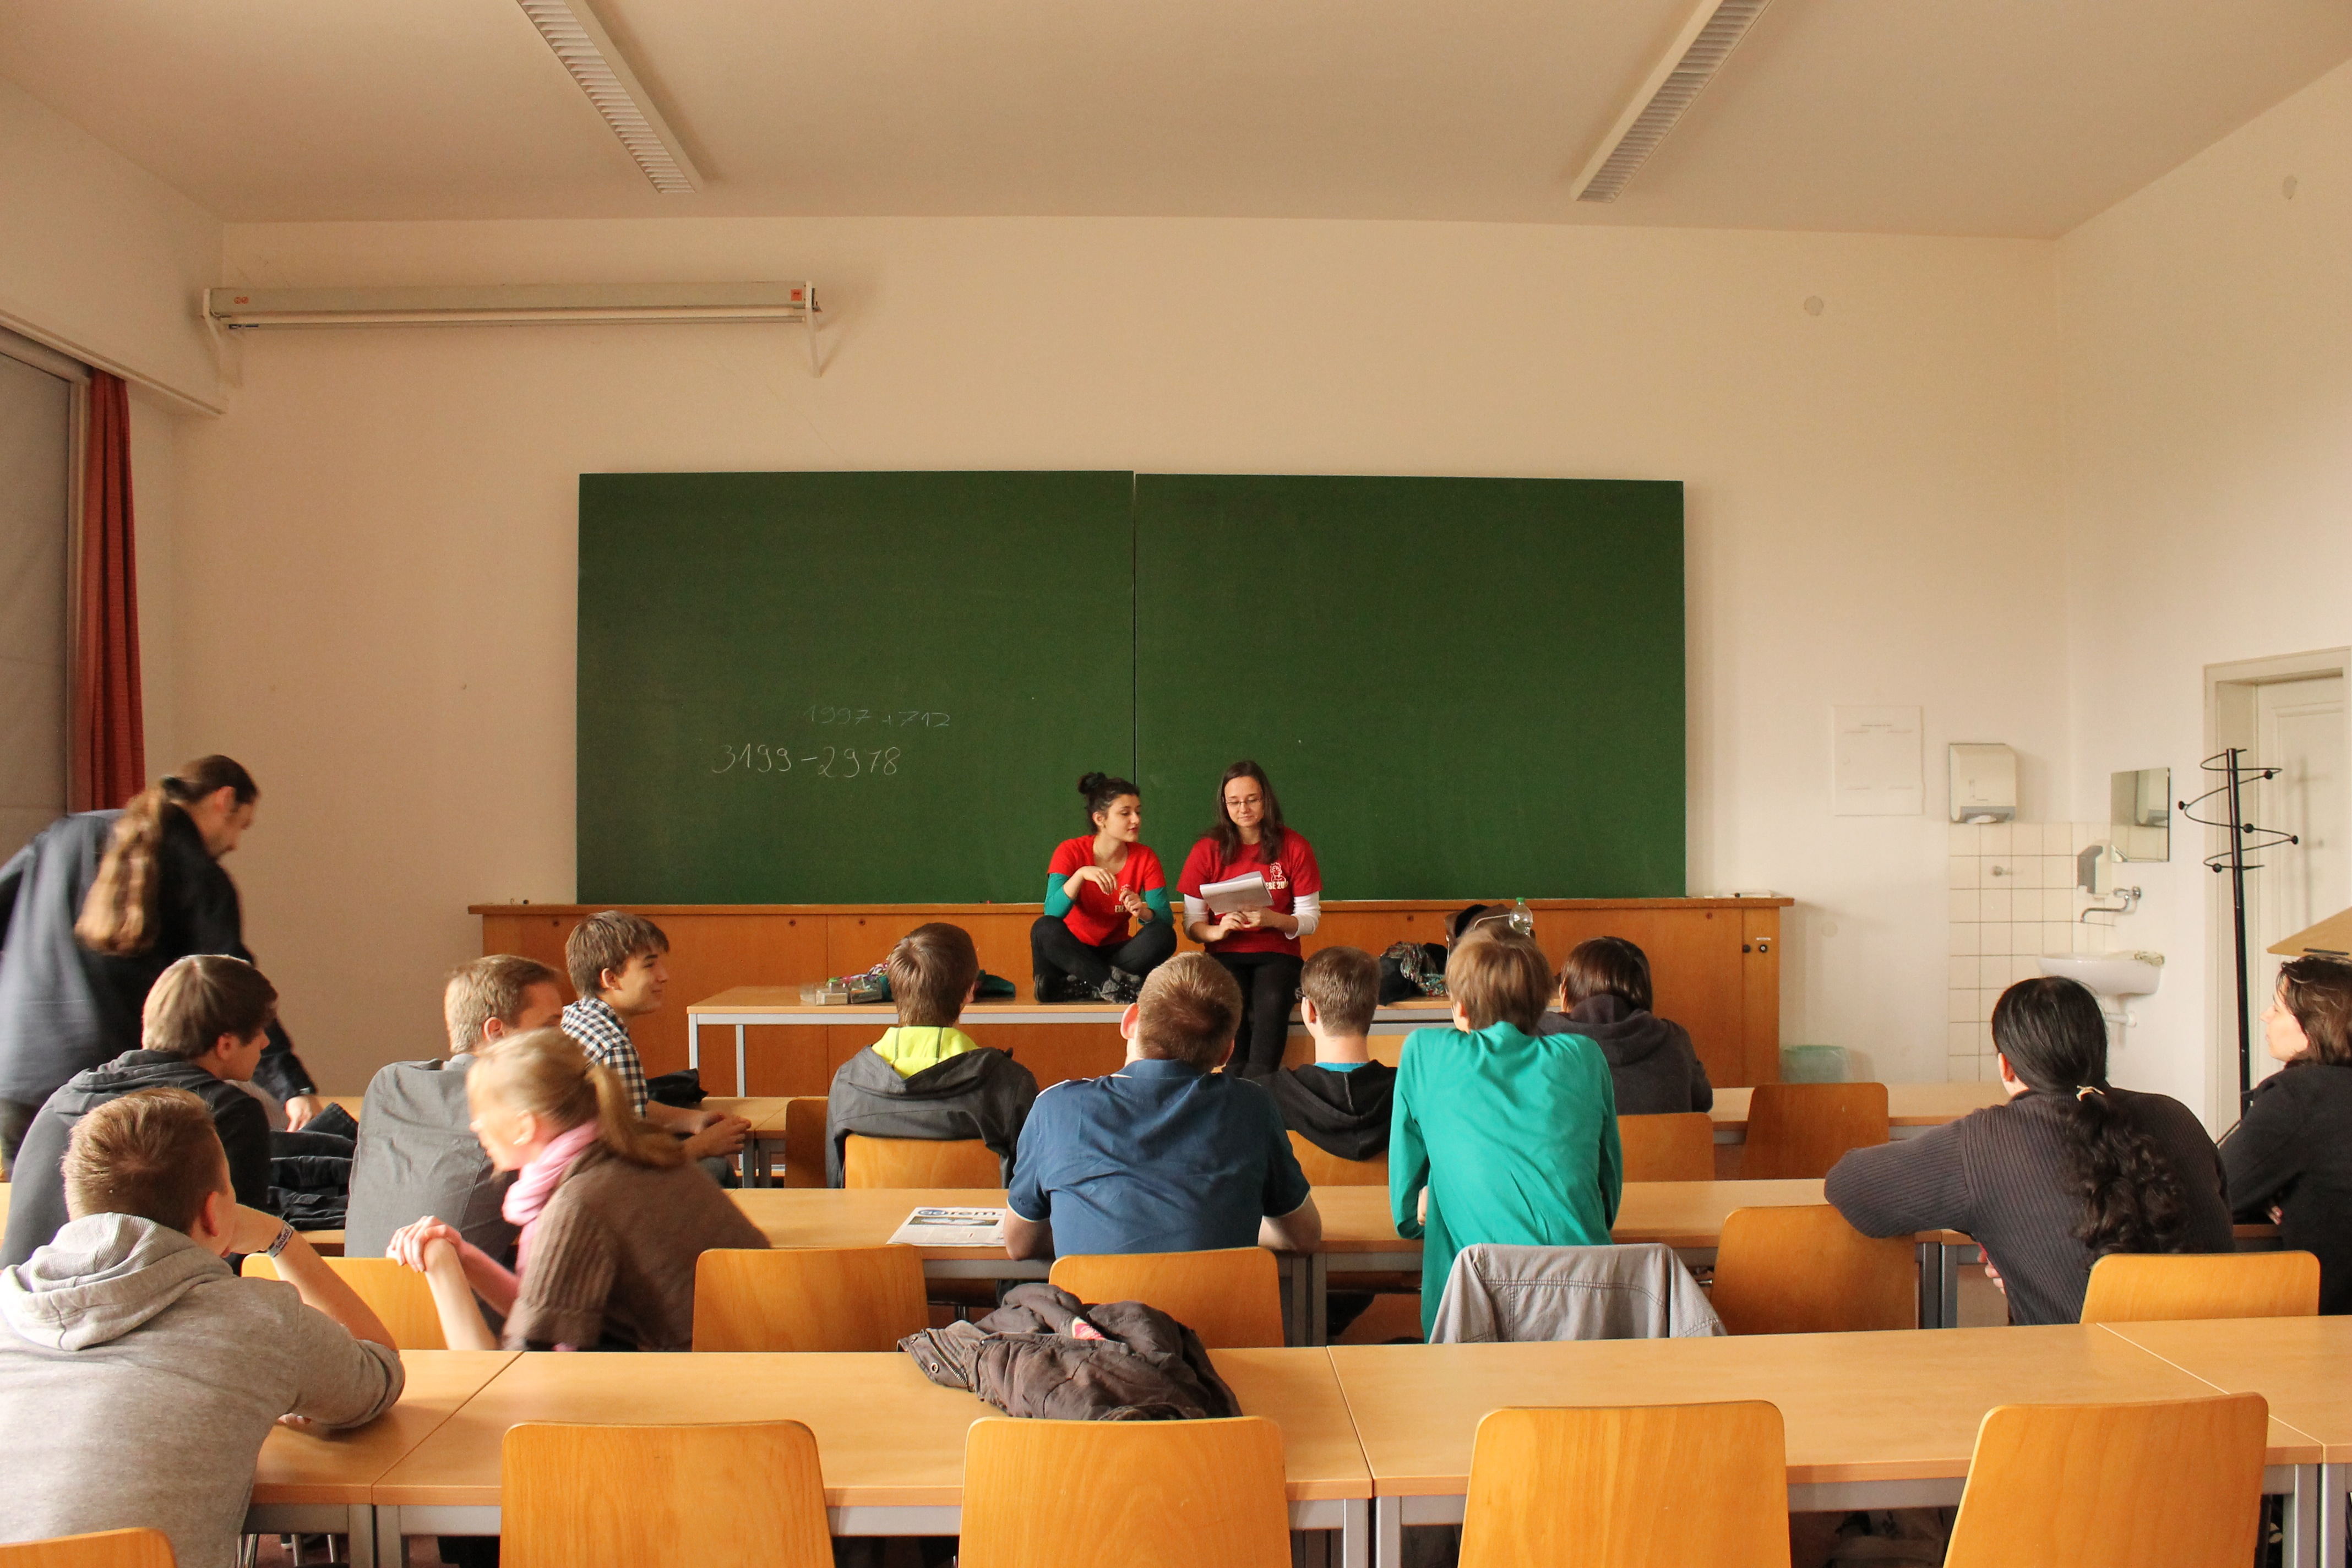
\includegraphics[width=\linewidth]{img/ese2013/tutorium.jpg}

\onecolumn
